\documentclass{bmvc2k}
\usepackage{url}

%% Enter your paper number here for the review copy
% \bmvcreviewcopy{??}

\title{PythonRobotics: a Python code collection of robotics algorithms}

% Enter the paper's authors in order
% \addauthor{Name}{email/homepage}{INSTITUTION_CODE}
\addauthor{Atsushi Sakai}{https://atsushisakai.github.io/}{1}

\addauthor{Daniel Ingram}{ingramds@appstate.edu}{2}

\addauthor{Joseph Dinius}{jdinius@inviarobotics.com}{3}

\addauthor{Karan Chawla}{karan@skyryse.com}{4}

\addauthor{Antonin Raffin}{antonin.raffin@ensta-paristech.fr}{5}

\addauthor{Alexis Paques}{Alexis@unmanned.life}{6}


% Enter the institutions
% \addinstitution{Name\\Address}
\addinstitution{
 University of California, Berkeley
}

\addinstitution{
 Appalachian State University
}

\addinstitution{
 inVia Robotics, Inc.
}

\addinstitution{
 Skyryse Inc.
}

\addinstitution{
 ENSTA ParisTech
}

\addinstitution{
 Unmanned Life
}


\runninghead{arXiv}{Robotics, Artificial Intelligence}

% Any macro definitions you would like to include
% These are not defined in the style file, because they don't begin
% with \bmva, so they might conflict with the user's own macros.
% The \bmvaOneDot macro adds a full stop unless there is one in the
% text already.
\def\eg{\emph{e.g}\bmvaOneDot}
\def\Eg{\emph{E.g}\bmvaOneDot}
\def\etal{\emph{et al}\bmvaOneDot}

%------------------------------------------------------------------------- 
% Document starts here
\begin{document}

\maketitle

\begin{abstract}
This paper describes an Open Source Software(OSS) project: PythonRobotics\cite{github}.
This is a Python code collection of robotics algorithms, especially focusing on autonomous navigation.
It aims for beginners of robotics to understand basic ideas of each algorithm.
In this project, the algorithms which are practical and widely used in both academia and industry are selected.
Each sample code is written by Python3 and only depends some standard modules for readability and trying to use easily.
It also provides intuitive animations to understand the behavior of the simulation.
In this paper, related works of this project, some key ideas about this OSS project, and brief structure of this repository are introduced.
Future works of this project are also discussed. 

\end{abstract}

%------------------------------------------------------------------------- 
\section{Introduction}

In recent years, autonomous navigation technologies have received a huge attention in many fields. 
For examples, autonomous driving\cite{pathplanning}, drone flight navigation, and other transportation systems.
The autonomous system is a system that can operate for long periods of time without any external control by human.

The autonomous navigation system needs a wide range of technologies.
It needs to know where am I (localization), where is safe (mapping), where to go (path planning), and how to go (path following). 
The autonomous system would not work correctly if any of these technologies is missing.

Educational materials for it are becoming more and more important for future developers to learn basic autonomous navigation technologies.
Because these autonomous technologies needs different technological backgrounds such as linear algebra, statics, probability theory, optimization theory, control theory, and sensing physics etc. 
It needs a lot of time to be familiar with these technological areas without good educational materials.

In this paper, an Open Source Software(OSS) project: PythonRobotics\cite{github} is described.
It aims for beginners of robotics to understand basic ideas of each algorithm.
This project provides a code collection of robotics algorithms, especially focusing on autonomous navigation. 
It is written in Python\cite{python} under MIT license\cite{mit}.
The unique point of this project has a lot of simulation animations that shows behaviors of each algorithm.
It helps for learners to understand it's fundamental ideas.
The readers can check the animations in the project page \url{https://atsushisakai.github.io/PythonRobotics/}.
The left figure in Fig.\ref{fig:github} shows the front image of the page.
All source codes of this project are provided at \url{https://github.com/AtsushiSakai/PythonRobotics}.

This project was started from Mar. 21 2016 as a self-learning project.
It already has over 3000 stars on GitHub, and the right figure in Fig.\ref{fig:github} shows the history of star counts graph using \cite{starhistory}.

\begin{figure}
\begin{tabular}{cc}
\bmvaHangBox{\fbox{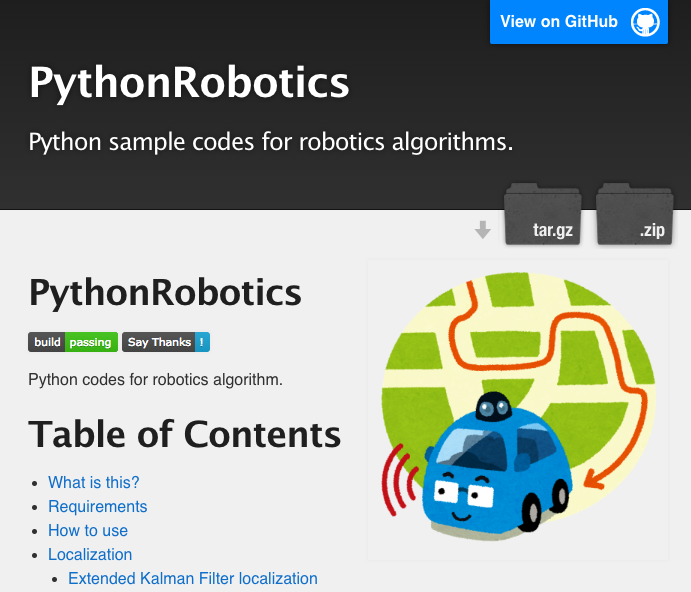
\includegraphics[width=5.3cm]{images/projectpage.png}}}&
\bmvaHangBox{\fbox{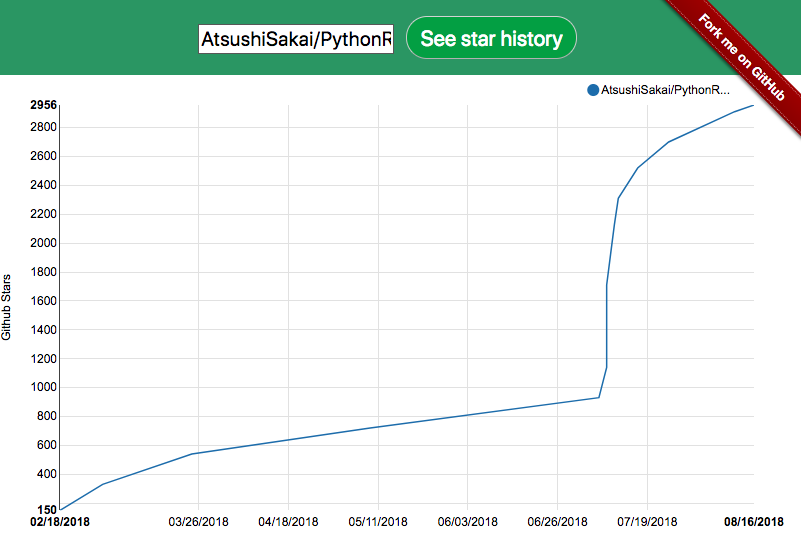
\includegraphics[width=6.6cm]{images/starhistory.png}}}\\

\end{tabular}
\caption{Right: PythonRobotics Project page, Left: GitHub star history graph using \cite{starhistory}}
\label{fig:github}
\end{figure}

This paper is organized as follows: Section 2 reviews the related works. The philosophy of this project is presented in Section 3. It's repository structure description and some technological backgrounds and simulation results are provided in Section 4. Conclusions and some future works are drawn in Section 5. 
Section 6 shows acknowledgements for all contributors and all supporters. 


\section{Related works}

There are great educational materials for learning autonomous navigation technologies.

S. Thrun et al. wrote a great text book "Probabilistic robotics" which is a bible of localization, mapping, simultaneous localization and mapping (SLAM) for mobile robotics\cite{PR}.
E. Frazzoli et al. wrote a great survey paper about path planning and control techniques for autonomous driving \cite{pathtracking}.
G. Bautista et al. wrote a survey paper focusing on path planning for automated vehicles\cite{pathplanning}.
J. Levinson wrote an overview paper about systems and algorithms towards fully autonomous driving\cite{Levinson2011}.

These papers helps readers to learn state of the arts autonomous navigation technologies.
However, it might be difficult to understand the basic ideas of the technologies and algorithms for beginners of robotics, because these papers doesn't include implementation examples such as sample codes.

Many universities provide great courses to learn robotics.
For example, University of Freiburg provides a introduction course of mobile robotics\cite{course1}.
Swiss Federal Institute of Technology in Zurich (ETH in Zurich) also provides a course of autonomous mobile robot\cite{course2} and robotics programming with Robot Operating System(ROS)\cite{course3}.

These lecture's notes also helps readers to learn the autonomous navigation technologies.
However, it might be difficult to understand the basic ideas of the technologies and algorithms for beginners of robotics if you are not a student of the class, because these lecture notes doesn't include implementation examples of robotics algorithms.

Robot Operating System (ROS) is a middle-ware for robotics software development\cite{ros}\cite{rospaper}.
ROS initially released from 2007, it became a defacto standard platform in many industries fields not only academia.
ROS includes basic navigation software such as Adaptive Monte Carlo Localization (AMCL package) and local path planner based on dynamic window approach, etc\cite{rosnavigation}.
Many autonomous navigation packages using ROS are also opened as an OSS.

The ROS packages are also useful to learn autonomous navigation algorithms.
However, it might has an issue sometimes, because of lacking of documentations about it's basic algorithm.
Also, it might be written by complicated programming languages such as C++ for calculation performance and platform reasons.
This is not good for focusing to learn robotics algorithms.

Udacity Inc, which is a online learning company founded by S. Thrun, et al, is providing great online courses of autonomous navigation and autonomous driving \cite{udacity}.
This course provide not only technical lectures, programming homework using Python.
It's learning strategy is great for understanding it's technical background.

PythonRobotics project has a similar concept to the Udacity's course.
It aims for beginners of robotics to understand basic technical ideas of each autonomous navigation algorithm using Python.
The details of concepts of this OSS project will be described in the next section. 

\begin{figure}
\begin{tabular}{cc}
\bmvaHangBox{\fbox{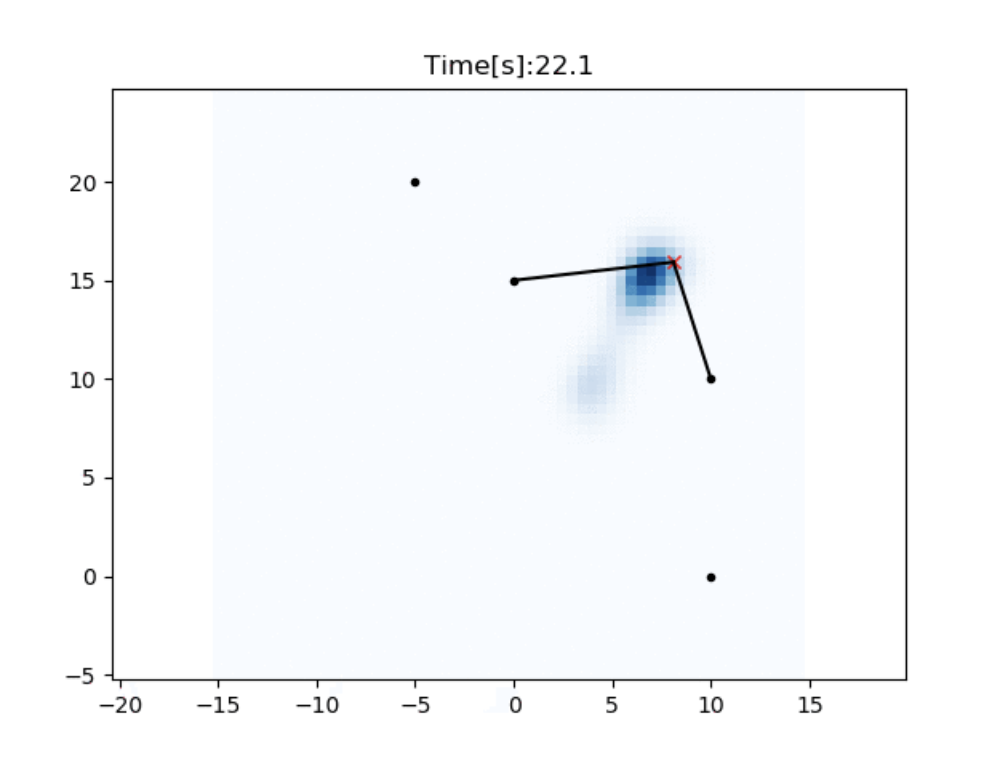
\includegraphics[width=5.9cm]{images/localization1.png}}}&
\bmvaHangBox{\fbox{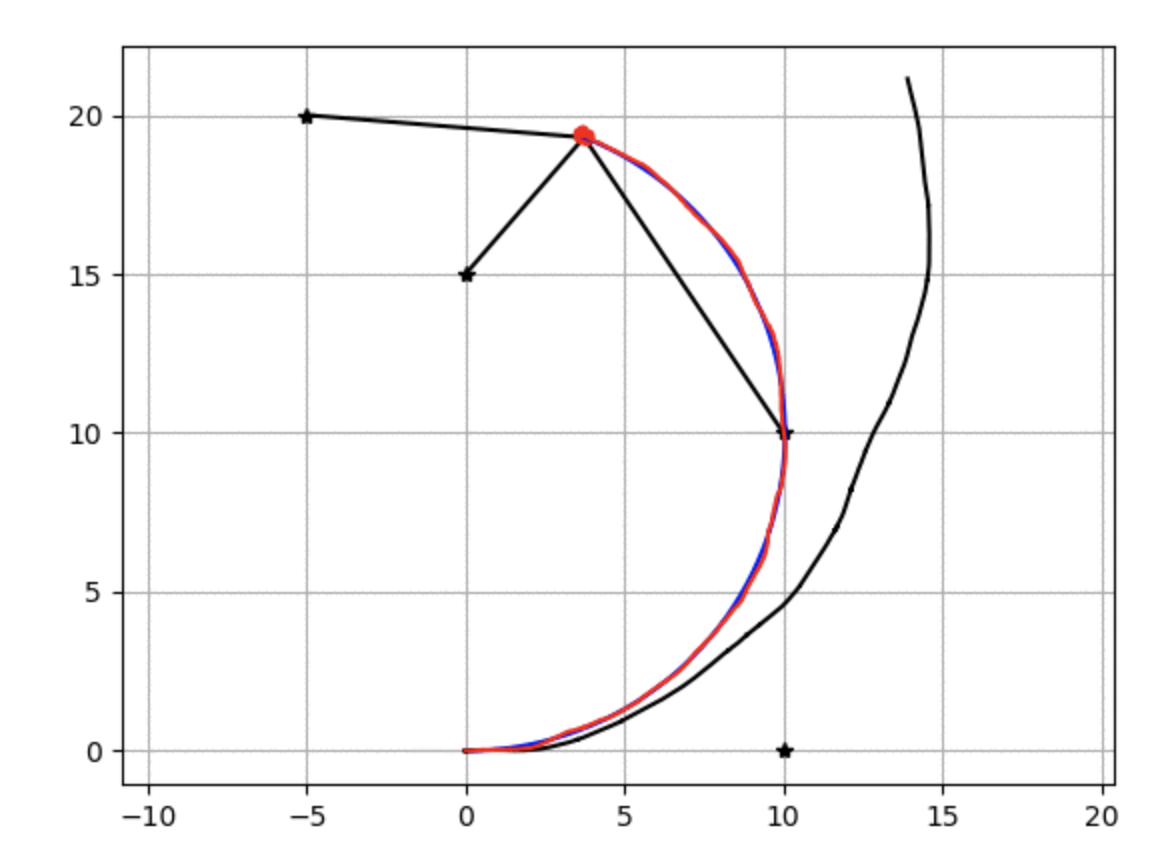
\includegraphics[width=6.2cm]{images/localization2.png}}}\\
Histogram filter&Particle filter
\end{tabular}
\caption{Localization simulation results}
\label{fig:localization}
\end{figure}

\section{Philosophy}
In this section, the philosophy of this project is described.
This project based on three main philosophies.

\subsection{Readability}
The first one is that the codes have to be easy to read for understanding each algorithm's basic idea.
This project aims for beginners of robotics to understand basic ideas of each algorithm. 
Therefore, the code have to be easy to read and understand the algorithm.
Programming language, Python\cite{python} is adopted in this project because it has good code readability and it allows us to focus on algorithm itself.
Python has great libraries for matrix operation, mathematical and scientific operation, and visualization.
These libraries also allows us to focus on algorithm itself.

\subsection{Practicality}
The second one is the algorithms which is widely used in academia and industry and practical are selected.
For example, Kalman filters and particle filter for localization, grid mapping for mapping, dynamic programming based approaches and sampling based approaches for path planning, and optimal control based approach for path tracking.

\subsection{Minimum dependency}
The last philosophy is minimum dependency.
It allows us to try the codes easily and to convert the Python codes to other programming languages such as C++, Java for practical usage.
Each sample code only depends some modules on Python3 as bellows.

\begin{itemize}
 \item numpy\cite{numpy} for matrix operation
 \item scipy\cite{scipy} for mathematics, science, and engineering computing
 \item matplotlib\cite{matplotlib} for visualization
 \item pandas\cite{pandas} for data analysis
 \item cvxpy\cite{cvxpy} for convex optimization
\end{itemize}

These modules are OSS and could be used for free.
This repository also doesn't depend on any commercial software.


\section{Repository structure}

In this section, the brief structure of this project is described.

This repository has five directories which means five technical categories in autonomous navigation, Localization, Mapping, SLAM, Path planning, and Path tracking.
Each directory includes several directories which has a sample code using different algorithms.

In the following subsections, some algorithms and some simulation examples described on each category.

\subsection{Localization}

Localization is an ability of a robot to know it's position and orientation with sensors such as GNSS and IMU.
In localization, Bayesian Filters such as Kalman filters, histogram filter, and particle filter are widely used\cite{PR}.
This repository includes some codes using the algorithms.
Fig.\ref{fig:localization} shows localization simulation results using histogram filter and particle filter.



\subsection{Mapping}
Mapping is an ability of a robot to understand surroundings with sensors such as LIDAR and imaging sensor.
Robots have to recognize obstacle positions and it' shape for obstacle avoidance.
In mapping, grid maping and machine learning algorithms are widely used\cite{PR}\cite{PRML}.
This repository includes sample codes using the algorithms.
Fig.\ref{fig:mapping} shows mapping simulation results using Grid mapping with 2D ray casting and 2D object clustering with k-means algorithm.

\begin{figure}
\begin{tabular}{cc}
\bmvaHangBox{\fbox{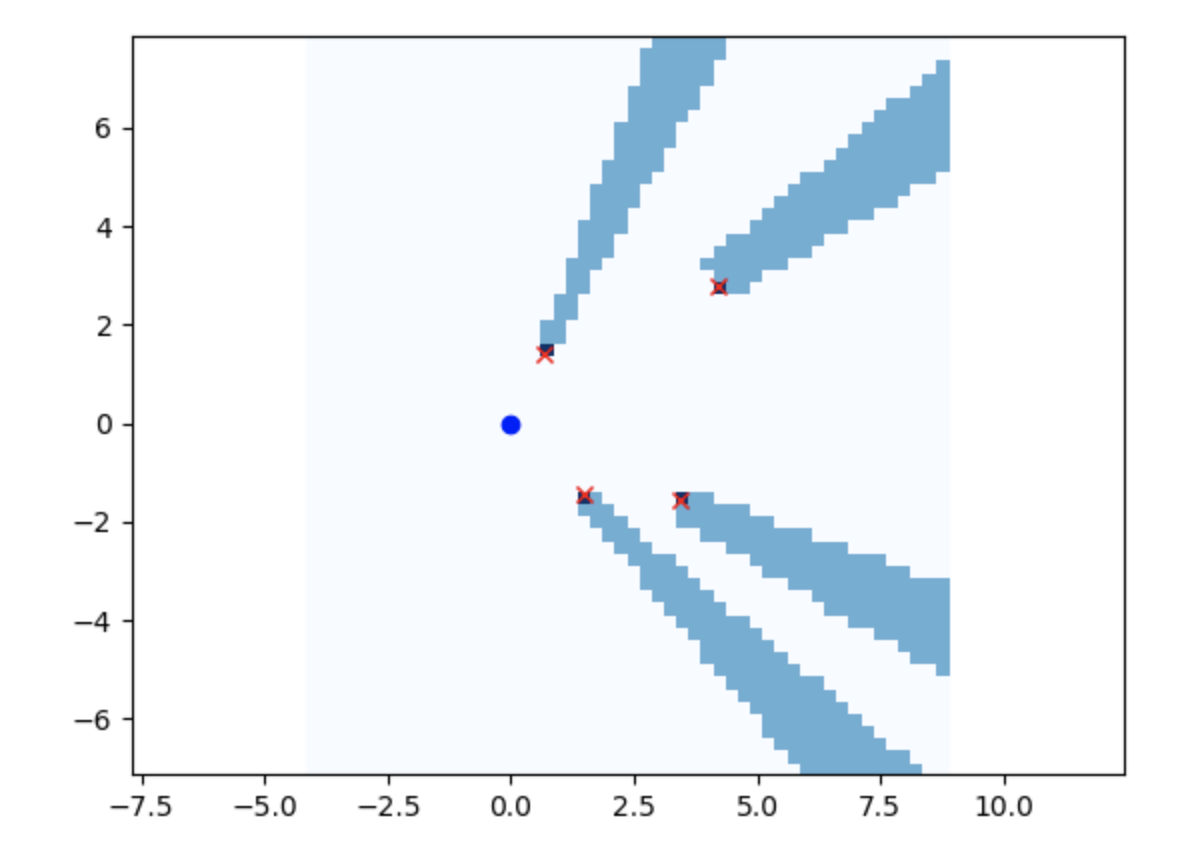
\includegraphics[width=6.0cm]{images/mapping1.png}}}&
\bmvaHangBox{\fbox{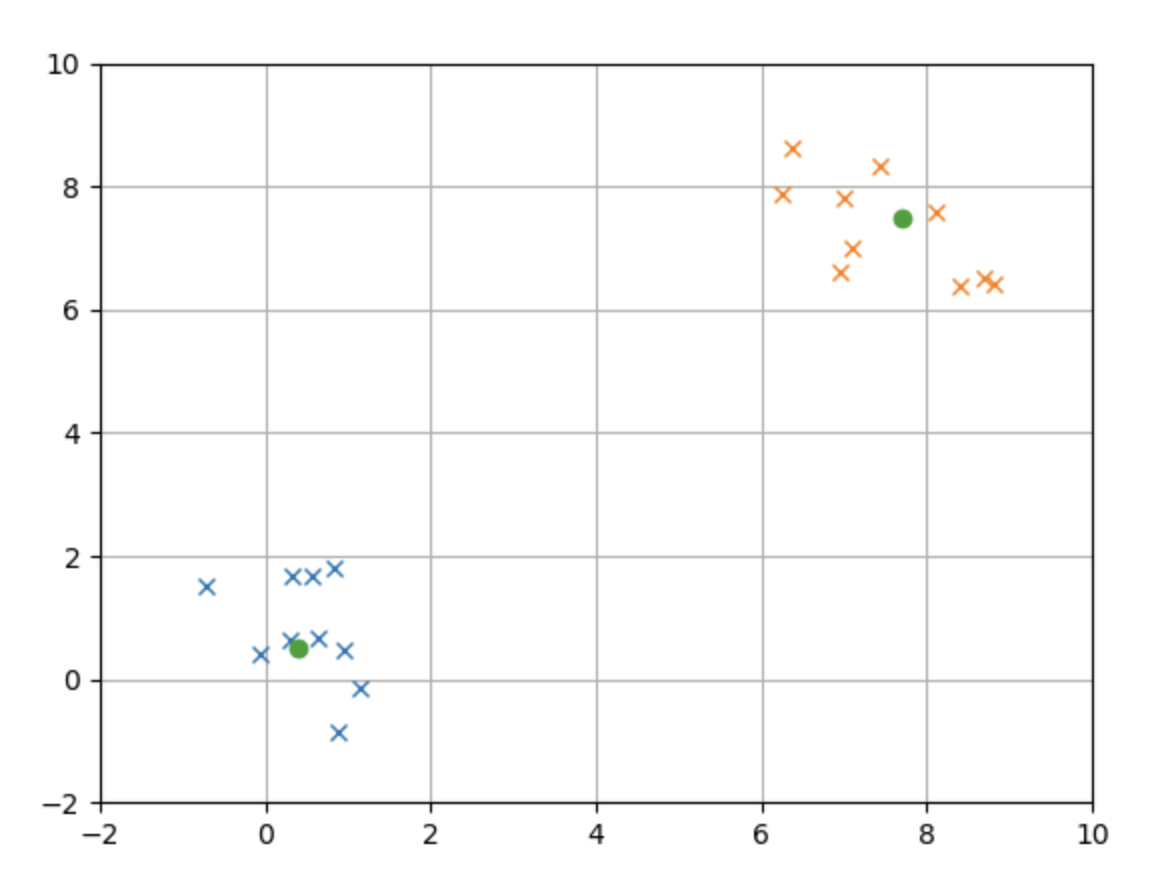
\includegraphics[width=5.7cm]{images/mapping2.png}}}\\
Grid mapping with 2D ray casting&2D object clustering with k-means algorithm
\end{tabular}
\caption{Mapping simulation results}
\label{fig:mapping}
\end{figure}

\subsection{SLAM}
Simultaneous Localization and Mapping (SLAM) is an ability to estimate the pose of a robot and the map of the environment at the same time.
SLAM problem is hard to solve, because a map is needed for localization and a good localization is needed for mapping, which is a kind of chicken and egg problem.
Popular SLAM solution methods include the extended Kalman filter, particle filter, and Fast SLAM algorithm\cite{PR}.
Fig.\ref{fig:slam} shows SLAM simulation results using Extended Kalman Filter and results using FastSLAM2.0\cite{PR}.

\begin{figure}
\begin{tabular}{cc}
\bmvaHangBox{\fbox{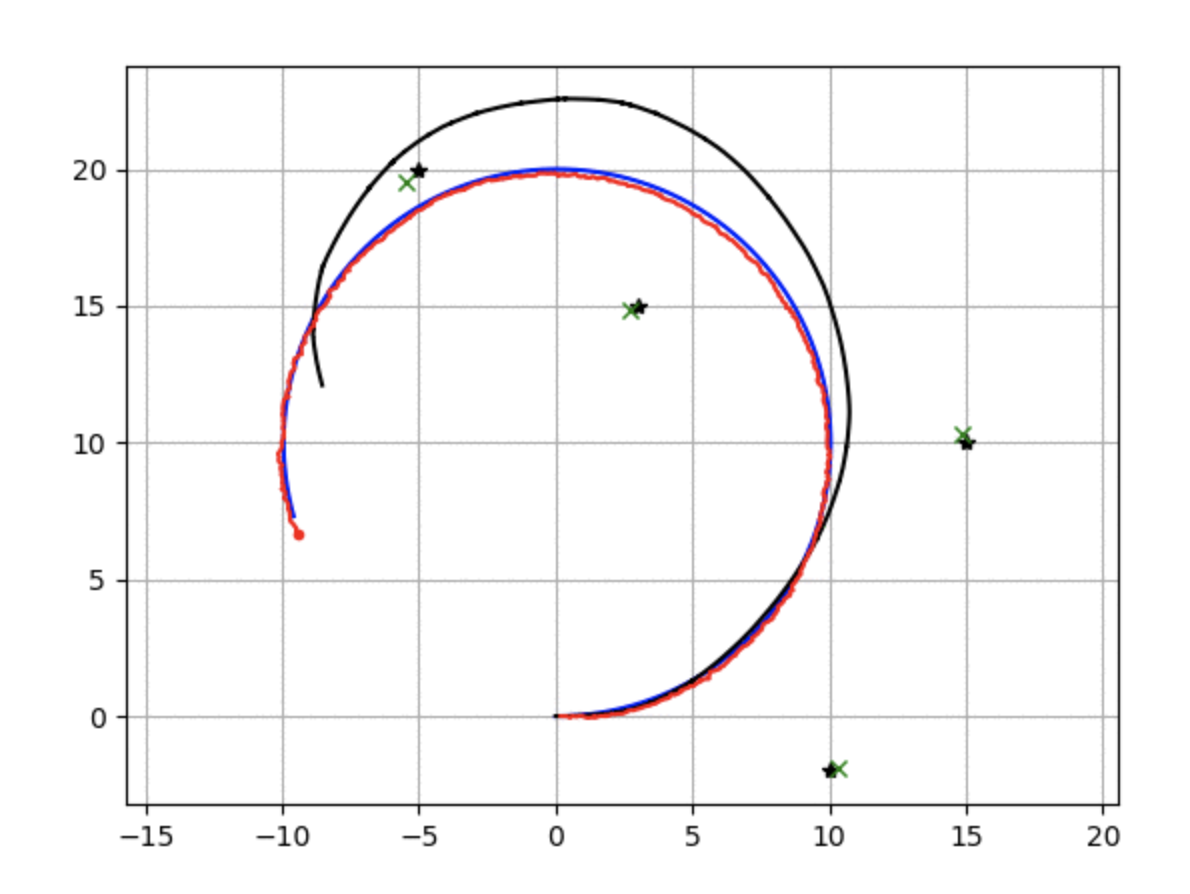
\includegraphics[width=6.0cm]{images/slam1.png}}}&
\bmvaHangBox{\fbox{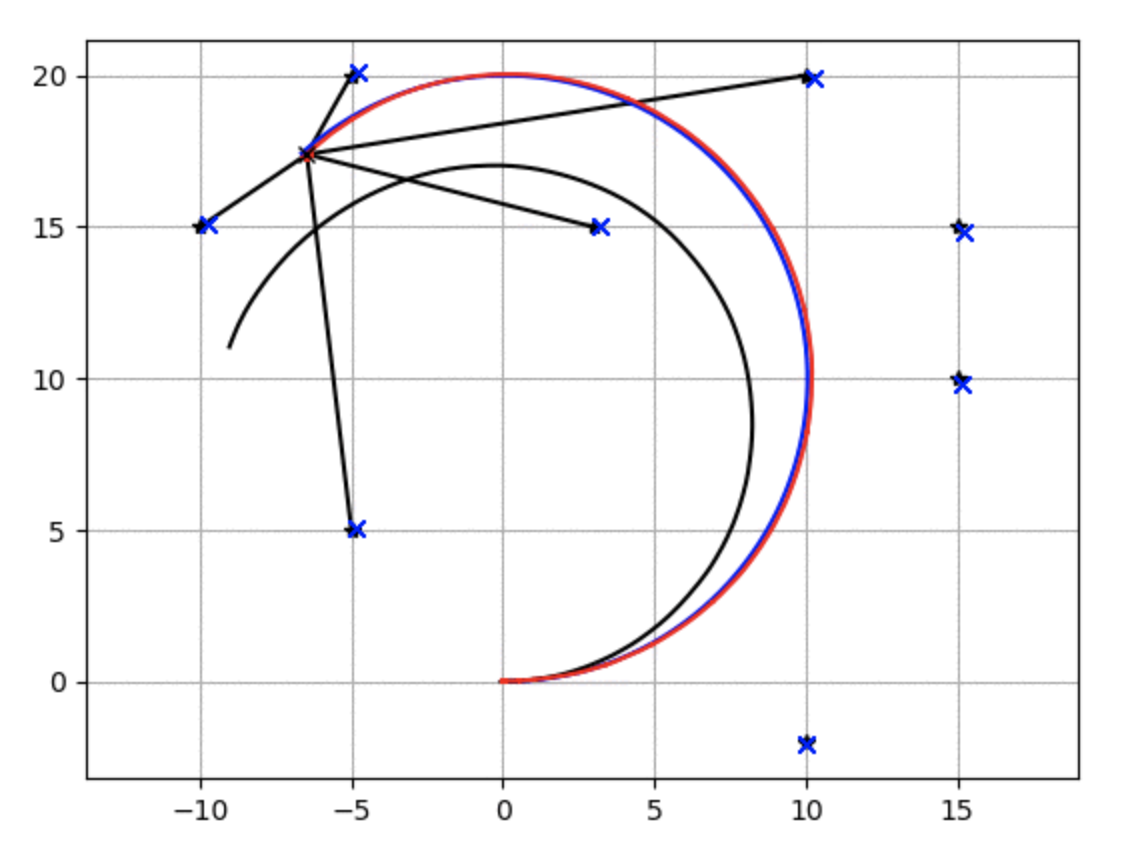
\includegraphics[width=6.0cm]{images/slam2.png}}}\\
Extended Kalman Filter based SLAM & FastSLAM 2.0 based SLAM
\end{tabular}
\caption{SLAM simulation results}
\label{fig:slam}
\end{figure}

\subsection{Path planning}

Path planning is an ability of a robot to search feasible and efficient path to the goal.
The path have to satisfy some constraints based on movement model and obstacle positions, and optimize some objective function such as time to goal and distance to obstacle etc.
In path planning, dynamic programming based approaches and sampling based approaches are widely used\cite{pathplanning}.
This project includes some sample codes using these algorithms.
Fig.\ref{fig:pathplan} shows simulation results of potential field path planning and LQR-RRT* path planning\cite{lqrrrt}.

\begin{figure}
\begin{tabular}{cc}
\bmvaHangBox{\fbox{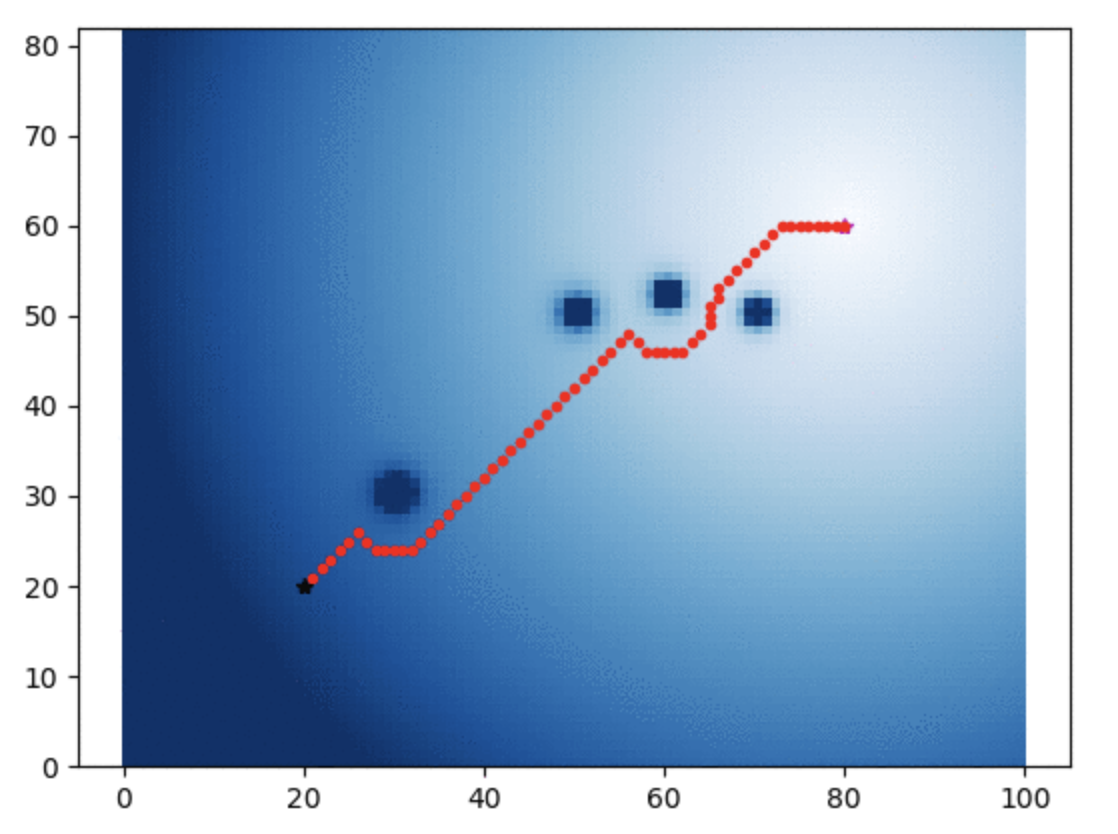
\includegraphics[width=6.0cm]{images/pathplan1.png}}}&
\bmvaHangBox{\fbox{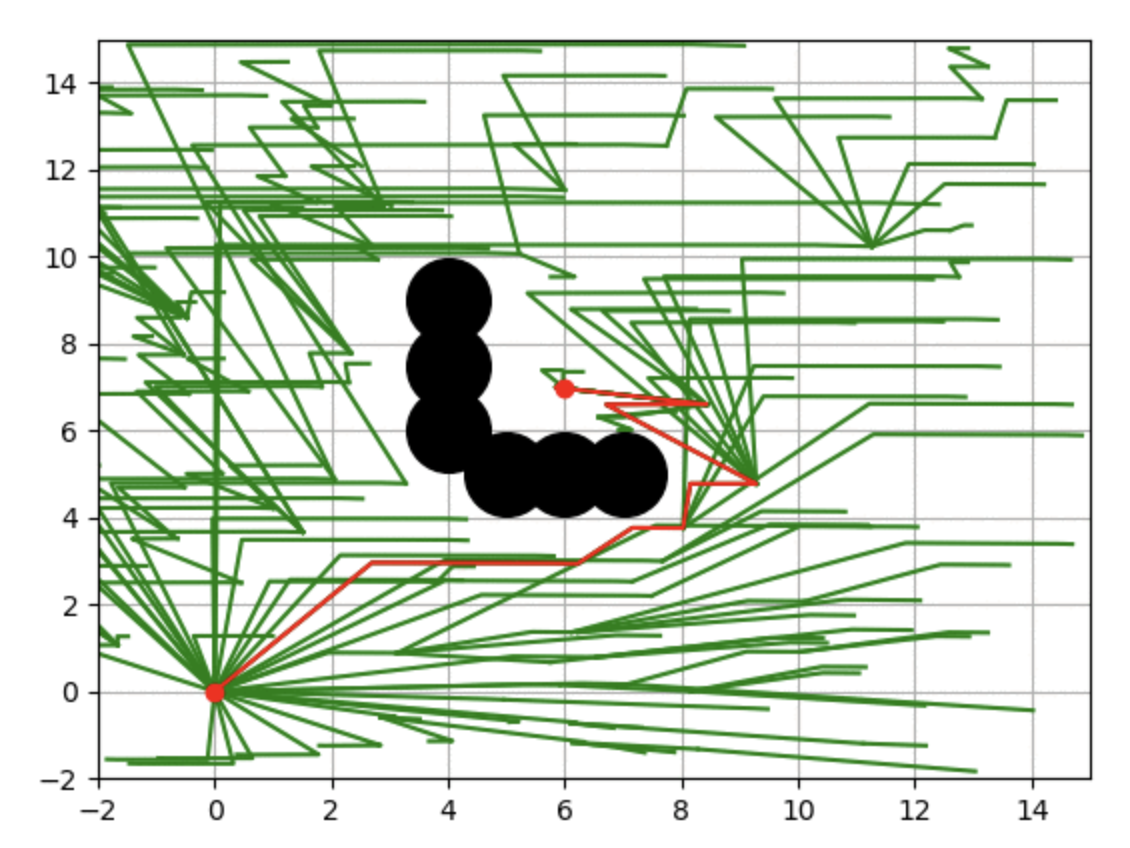
\includegraphics[width=6.0cm]{images/pathplan2.png}}}\\
Potential Field path planning & LQR-RRT* path planning\cite{lqrrrt}
\end{tabular}
\caption{Path planning simulation results}
\label{fig:pathplan}
\end{figure}

\subsection{Path tracking}
Path tracking is an ability of a robot to follow the reference path generated by path planning algorithms.
The role of the path tracking controller is to stabilize to the reference path or trajectory which has modeling error and other forms of uncertainty. 
In path tracking, feedback control techniques and optimization based control techniques are widely used\cite{pathplanning}.
This project includes some sample codes using these algorithms.
Fig.\ref{fig:pathplan} shows simulations using rear wheel feedback steering control and PID speed control, and iterative linear model predictive path tracking control\cite{lqrrrt}.

\begin{figure}
\begin{tabular}{cc}
\bmvaHangBox{\fbox{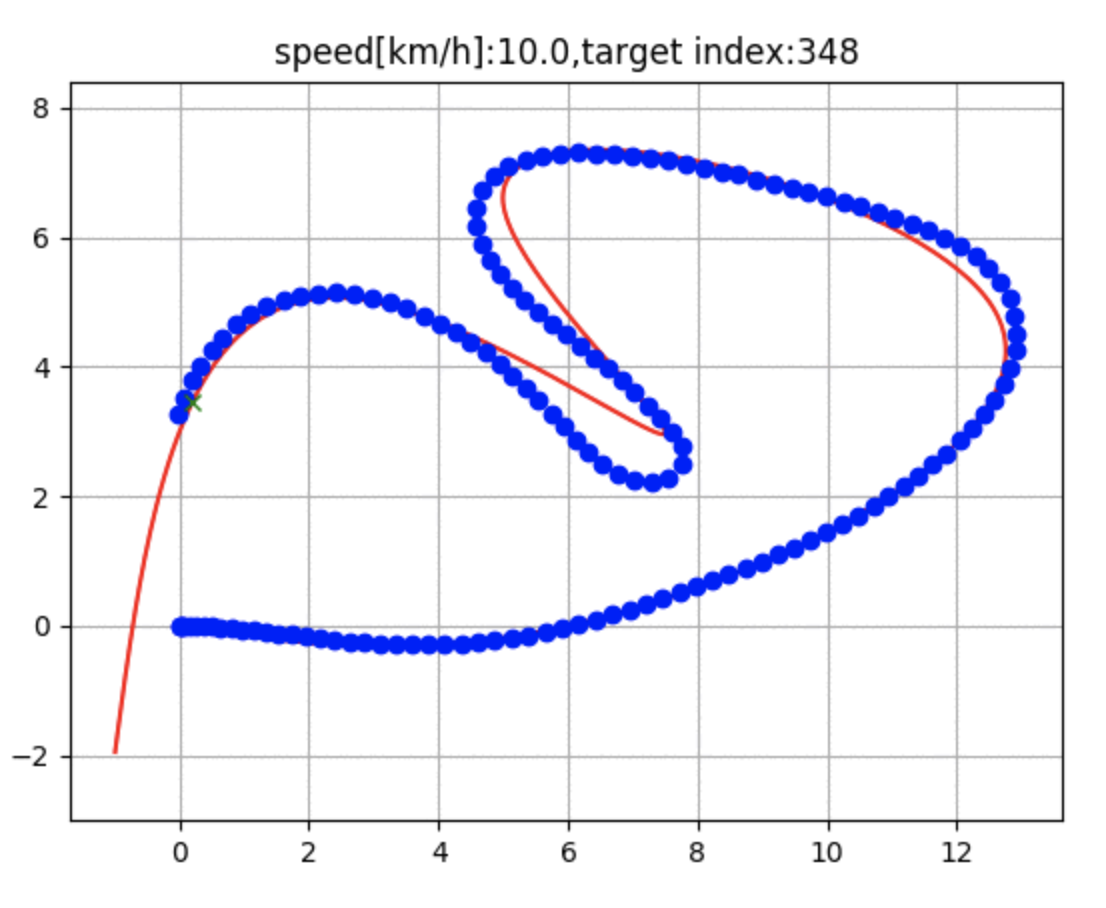
\includegraphics[width=6.0cm]{images/path_tracking1.png}}}&
\bmvaHangBox{\fbox{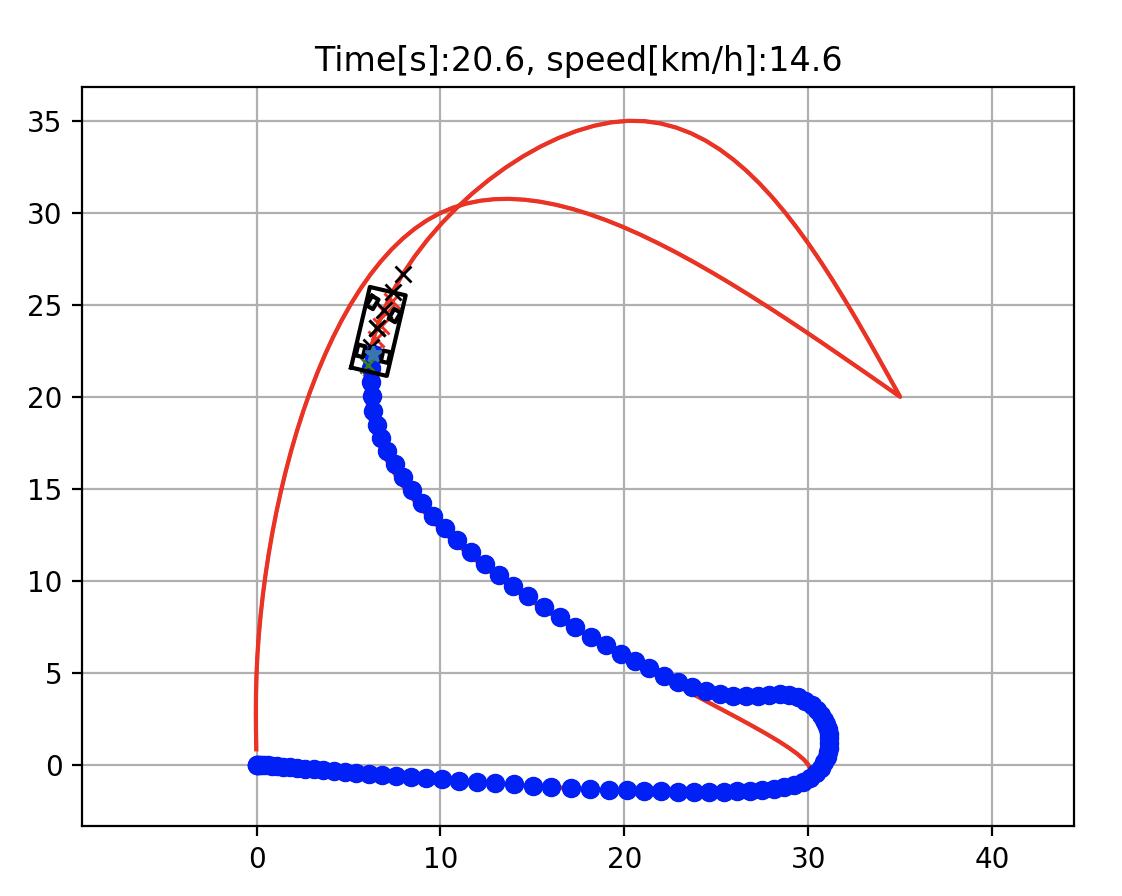
\includegraphics[width=6.2cm]{images/path_tracking2.png}}}\\
Rear wheel feedback steering control \\ and PID speed control \cite{pathtracking}& Iterative linear model predictive control
\end{tabular}
\caption{Path tracking simulation results}
\label{fig:pathplan}
\end{figure}

%------------------------------------------------------------------------- 
\section{Conclusion and future work}

In this paper, We introduced an OSS project, PythonRobotics which is a Python code collection of robotics algorithms, especially for autonomous navigation.
Related works of this project, some key ideas about this OSS project, and brief structure of this repository and some simulation results were described. 

The future works of this project are as followed: 

\begin{itemize}
 \item Adding technical and mathematical documentation using Jupyter notebook\cite{JupyterNotebook}.  
 \item Adding simple image processing sample codes for autonomous navigation only using OpenCV\cite{opencv}.
 \item Adding simple multi-robots simulations for autonomous navigation.
\end{itemize}

If readers were interested in these future projects, contributions are welcome.
Readers can also support this project financially via Patreon\cite{patreon}.

%------------------------------------------------------------------------
\section{Acknowledgments}

We appreciate all contributors: Atsushi Sakai\cite{auther6}, Daniel Ingram\cite{auther1}, Joe Dinius\cite{auther2}, Karan Chala\cite{auther3}, Antonin RAFFIN\cite{auther4}, and Alexis Paques\cite{auther6}.

We also appreciate all robotics lovers who give a star to this repository in GitHub.


\bibliography{egbib}
\end{document}
